% Copyright 2011-2014 David Hadka.  All Rights Reserved.
%
% This file is part of the MOEA Framework User Manual.
%
% Permission is granted to copy, distribute and/or modify this document under
% the terms of the GNU Free Documentation License, Version 1.3 or any later
% version published by the Free Software Foundation; with the Invariant Section
% being the section entitled "Preface", no Front-Cover Texts, and no Back-Cover
% Texts.  A copy of the license is included in the section entitled "GNU Free
% Documentation License".

\chapter{Parallelization}
\label{chpt:parallelization}

When we first introduced the \java{Executor} class in \chptref{chpt:executor}, we demonstrated the \java{distributeOnAllCores()} method as a way to automatically and seamlessly distribute the evaluation across all cores in your local computer.  This section shows how to expand this simple distributed computing methods to large-scale cloud and high-performance computing systems.  This form of parallelization is typically called ``master-slave'' processing, where the MOEA is run on a single node called the master and all problem evaluations are distributed to one or more slave nodes for processing.

In order for this form of parallelization to work, the algorithm must be naturally parallelizable.  To be naturally parallelizable, the algorithm must avoid querying the evaluation results (i.e., the objectives and constraint values) prior to evaluating all solutions.  This is typically achieved by designing an algorithm to invoke the \java{evaluateAll(...)} method.  If this condition holds, then the MOEA Framework will automatically detect that the algorithm is parallelizable and enable master-slave processing.  A simple way to determine if an algorithm is parallelizable is to use the \java{distributeOnAllCores()} method in the \java{Executor} and checking the CPU usage of each core. 

Many of the algorithms provided by the MOEA Framework are parallelizable (e.g., NSGA-II, $\epsilon$-NSGA-II, NSGA-III, GDE3) but others like are not (e.g., $\epsilon$-MOEA, MOEA/D).

\section{JPPF}
\begin{wrapfigure}{l}{4cm}
  
\includegraphics[width=4cm]{jppf.png}
\end{wrapfigure}
JPPF is a Java framework for parallel processing licensed under the Apache license, version 2, which is a free and open-source license.  This section demonstrates distributing the problem evaluations using JPPF.  This example was tested using JPPF version 4.2.5.  For the purposes of this exercise, we will run all slave nodes on a single computer.  Please refer to the JPPF documentation for information on running nodes on multiple computers.

To begin, first download the Server/Driver, Node, and Application Template distributions from \webpage{http://www.jppf.org/} and unzip the files to any location on your computer.  Next, create a new project in your Java development environment (e.g., Eclipse or NetBeans).  Add to the project the MOEA Framework and JPPF JAR files located in the \folder{MOEAFramework-%VERSION%/lib} and \folder{JPPF-4.2.5-application-template/lib} folders, respectively.  If using Eclipse, the project folder should appear similar to \figref{fig:jppfProjectSetup}.

\begin{figure}
  \center
  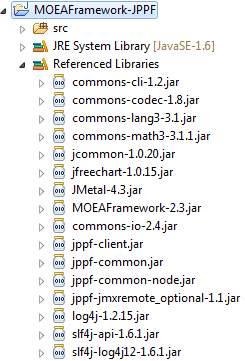
\includegraphics{jppfProjectSetup.png}
  \caption{Screenshot of an Eclipse project with the JPPF and MOEA Framework JAR files included.}
  \label{fig:jppfProjectSetup}
\end{figure}  

In this example, we will create a simple test problem and artificially make it computationally expensive by adding a long-running loop.  Create a new Java class file called \file{ParallelProblem.java} with the following code:

\begin{lstlisting}[language=Java]
import java.io.Serializable;

import org.moeaframework.core.Problem;
import org.moeaframework.core.Solution;
import org.moeaframework.core.variable.EncodingUtils;

public class ParallelProblem implements Problem, Serializable {

	private static final long serialVersionUID = 5790638151819130066L;

	@Override
	public String getName() {
		return "ParallelProblem";
	}
	
	@Override
	public int getNumberOfVariables() {
		return 1;
	}

	@Override
	public int getNumberOfObjectives() {
		return 2;
	}
	
	@Override
	public int getNumberOfConstraints() {
		return 0;
	}

	@Override
	public void evaluate(Solution solution) {
		long start = System.currentTimeMillis();
		double x = EncodingUtils.getReal(solution.getVariable(0));
		
		// simulate time-consuming evaluation
		for (long i = 0; i < 500000000; i++);
		
		solution.setObjective(0, Math.pow(x, 2.0));
		solution.setObjective(1, Math.pow(x - 2.0, 2.0));
		
		System.out.println("Elapsed time: " + (System.currentTimeMillis() - start));
	}

	@Override
	public Solution newSolution() {
		Solution solution = new Solution(1, 2);
		solution.setVariable(0, EncodingUtils.newReal(-10.0, 10.0));
		return solution;
	}
	
	@Override
	public void close() {
		//do nothing
	}

}
\end{lstlisting}

Note that this class implements the \java{Serializable} interface.  This is a required step for parallelization.  Implementing the \java{Serializable} class allows the Java class to be encoded and transmitted across a network.  To make a serializable class, all one needs to do is add \java{implements Serializable} after the class name, as shown in this example.

Next, create another Java class called \file{JPPFExample.java} with the following code:

\begin{lstlisting}[language=Java]
import org.jppf.client.JPPFClient;
import org.jppf.client.concurrent.JPPFExecutorService;
import org.moeaframework.Executor;
import org.moeaframework.core.NondominatedPopulation;

public class JPPFExample {

	public static void main(String[] args) {
		JPPFClient jppfClient = null;
		JPPFExecutorService jppfExecutor = null;

		try {
			jppfClient = new JPPFClient();
			jppfExecutor = new JPPFExecutorService(jppfClient);
			
			// setting the batch size is important, as JPPF will only
			// run one job at a time from a client; the batch size
			// lets us group multiple evaluations (tasks) into a
			// single job
			jppfExecutor.setBatchSize(100);
			jppfExecutor.setBatchTimeout(100);
			
			long start = System.currentTimeMillis();

			NondominatedPopulation result = new Executor()
					.withProblemClass(ParallelProblem.class)
					.withAlgorithm("NSGAII")
					.withMaxEvaluations(10000)
					.distributeWith(jppfExecutor)
					.run();
			
			System.out.println("Solutions found: " + result.size());
			System.out.println("Total elapsed time: " + 
						((System.currentTimeMillis() - start) / 1000) +
						" seconds");
		} catch(Exception e) {
			e.printStackTrace();
		} finally {
			if (jppfExecutor != null) {
				jppfExecutor.shutdown();
			}

			if (jppfClient != null) {
				jppfClient.close();
			}
		}
	}
	
}
\end{lstlisting}

With these two files created, we can now test this example.  Prior to running the Java code we just created, you will need to start the JPPF driver and one or more JPPF nodes.  To start the driver, run the \file{JPPF-4.2.5-driver/startDriver.bat} program.  To start a local node, run the \file{JPPF-4.2.5-node/startNode.bat} program.  You should see two command prompt windows appear.  Finally, run the \java{JPPFExample} class we just created.  If all works as intended, your computer should now be running at or near $100\%$ CPU utilization.

During our testing, we found that running this example on a single local core with no parallelization takes approximately $1,687$ seconds while running on four local cores takes approximately $545$ seconds.  This results in a speedup of $3.1$.  We lose some speedup due to communication overhead between the master and slave nodes, but still obtain a reasonable speedup.

\section{Conclusion}
This chapter provided an introduction to parallel computing with the MOEA Framework.  We will continue to expand on this section in future releases to provide examples of other parallel libraries and parallelization techniques.